\subsection{Layer 4 (Transport)}
\subsection*{Aufgaben}
\begin{itemize}
	\item Anwendungen identifizieren
	\item Segmentierung
	\item ev. Flusskontrolle, Verbindungsauf- \& abbau
	\item Kommunikation mit L3 \& L5
\end{itemize}

\subsection*{Protkolle} 
\begin{itemize}
	\item TCP (Transmission Control Protocol)
	\item UDP (User Datagram Protocol)
\end{itemize}

\begin{table}[H]
	\begin{tabular}{l|l}
		\multicolumn{1}{c|}{TCP} & \multicolumn{1}{c}{UDP} \\
		\hline
		Anwendungen identifizieren (Ports) & Anwendungen identifizieren (Ports) \\
		Segmentierung & Segmentierung \\
		Verbindungen auf- bzw abbauen &  \\
		Segmente ordnen &  \\
		wiederholtes Senden &  \\
		Flusskontrolle & 
	\end{tabular}
\end{table}
\textbf{TCP:} HTTP (80)/HTTPS (443), SMTP (25), POP (110), IMAP (143), Telnet (23), SSH (22), FTP (20/21),... \\
\textbf{UDP:} DNS (53), DHCP (67/68), VoIP, Streaming,...

\subsection*{Ports}
Der Port ist eine 16-Bit Zahl $\rightarrow$ $2^{16} = 65.536$ \\
Der Port identifiziert die Anwendung, sowohl beim Server als auch beim Client.

\subsection*{Gruppe von Ports}
\begin{table}[H]
	\begin{tabular}{rc}
		Well-Known-Ports & 0 - 1.023 \\
		Registered-Ports & 1.024 - 49.151 \\
		Private Ports & 49.152 - 65.535
	\end{tabular}
\end{table}

\subsection*{L4-Adressierung}
\begin{figure}[H]
	\centering
	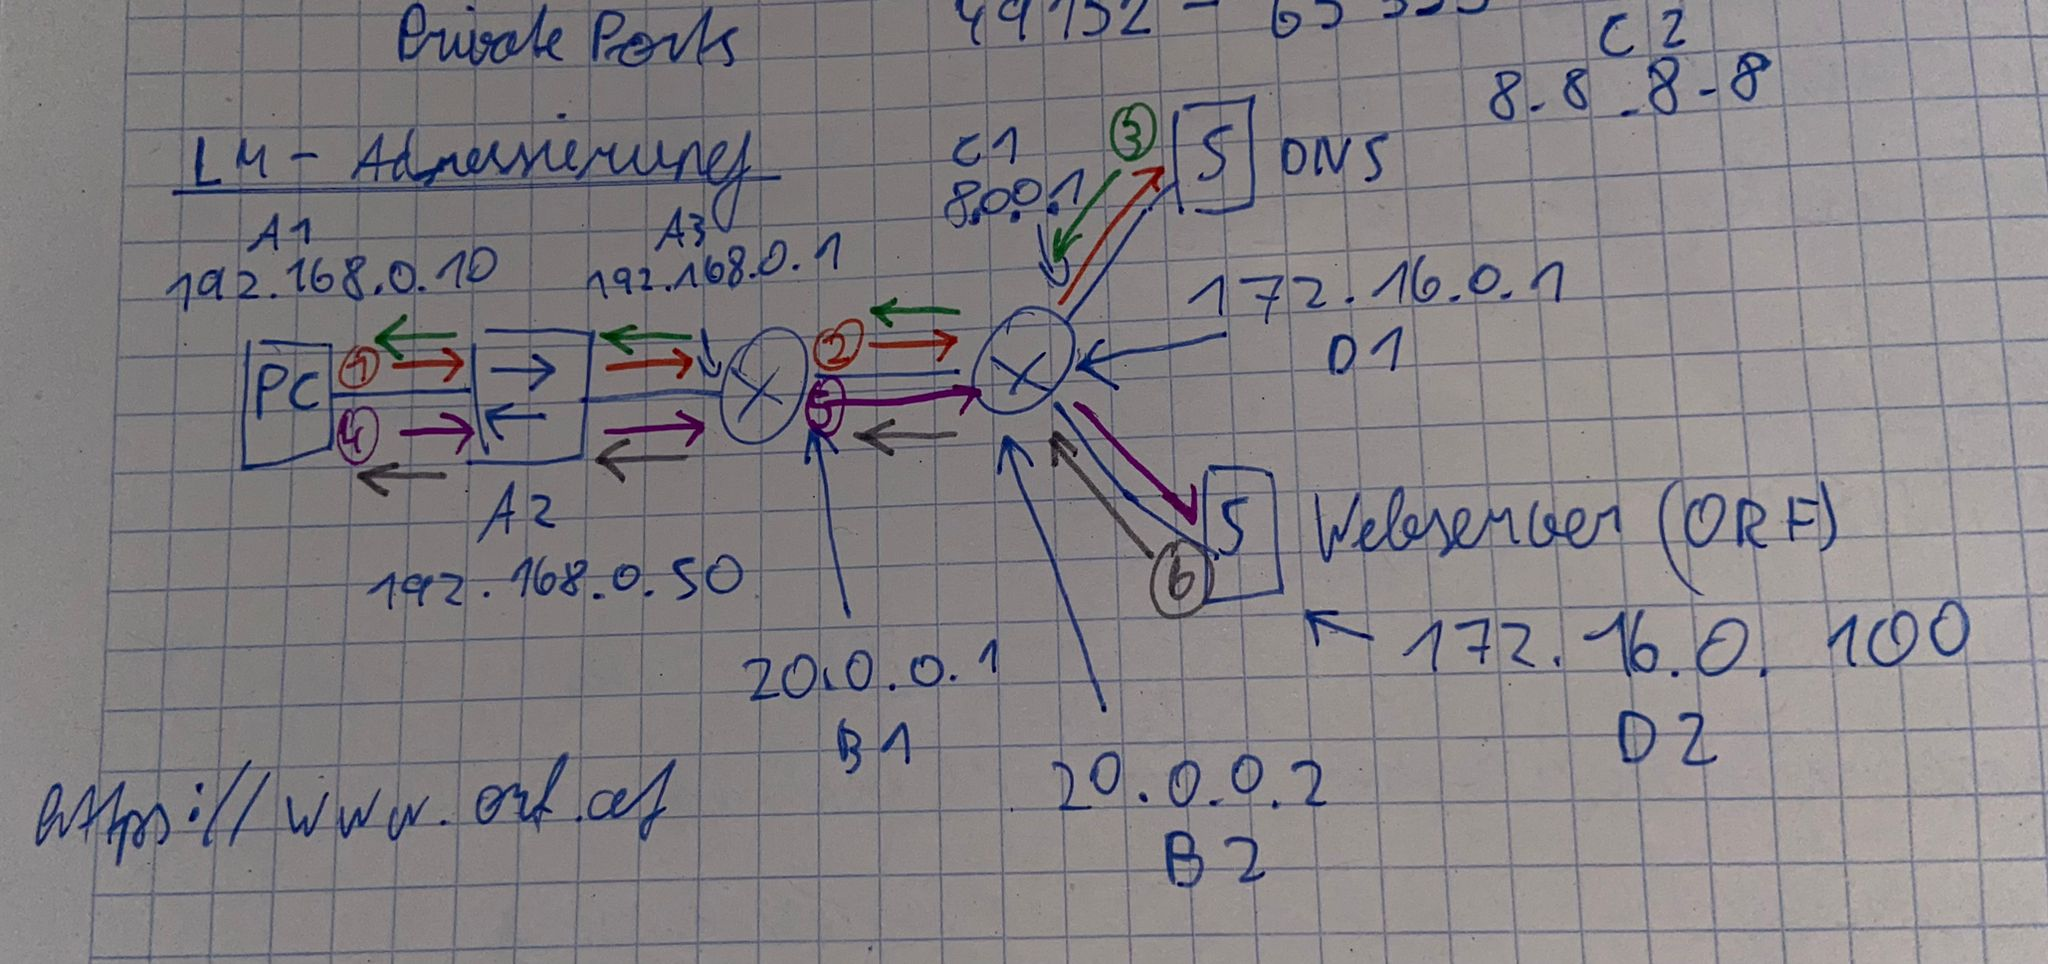
\includegraphics[width=1.0\linewidth]{figures/l4_addr.jpeg}
	\caption{L4-Adressierung}
\end{figure}

\begin{table}[H]
	\begin{tabular}{c|ccllll}
		& \multicolumn{2}{c}{L2 (MAC)} & \multicolumn{2}{c}{L3 (IP)} & \multicolumn{2}{c}{L4 (Ports)} \\
		& \multicolumn{1}{c}{Source} & \multicolumn{1}{c}{Destination} & \multicolumn{1}{c}{Source} & \multicolumn{1}{c}{Destination} & \multicolumn{1}{c}{Source} & \multicolumn{1}{c}{Destination} \\
		\hline
		1 & A1 & A3 & 192.168.0.10 & 8.8.8.8 & 53.722 & 53 \\
		2 & B1 & B2 & 192.168.0.10 & 8.8.8.8 & 53.722 & 53 \\
		3 & C2 & C1 & 8.8.8.8 & 192.168.0.10 & 53 & 53.722 \\
		4 & A1 & A3 & 192.168.0.10 & 172.16.0.100 & 60.112 & 443 \\
		5 & B1 & B2 & 192.168.0.10 & 172.16.0.100 & 60.112 & 443 \\
		6 & D2 & D1 & 172.16.0.100 & 192.168.0.10 & 443 & 60.112
	\end{tabular}
\end{table}

\subsection*{TCP}
\textbf{Verbindungsaufbau: Drei-Wege-Handshake}
\begin{figure}[H]
	\centering
	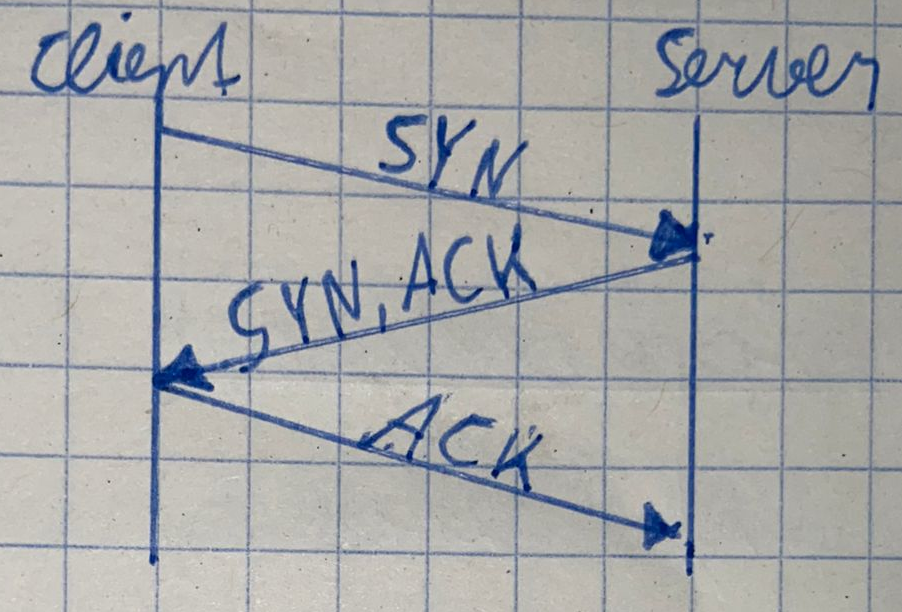
\includegraphics[width=0.8\linewidth]{figures/tcp_3wh.png}
	\caption{TCP 3-Way-Handshake}
\end{figure}

\textbf{Verbindungsabbau: Zwei-Wege-Handshake}
\begin{figure}[H]
	\centering
	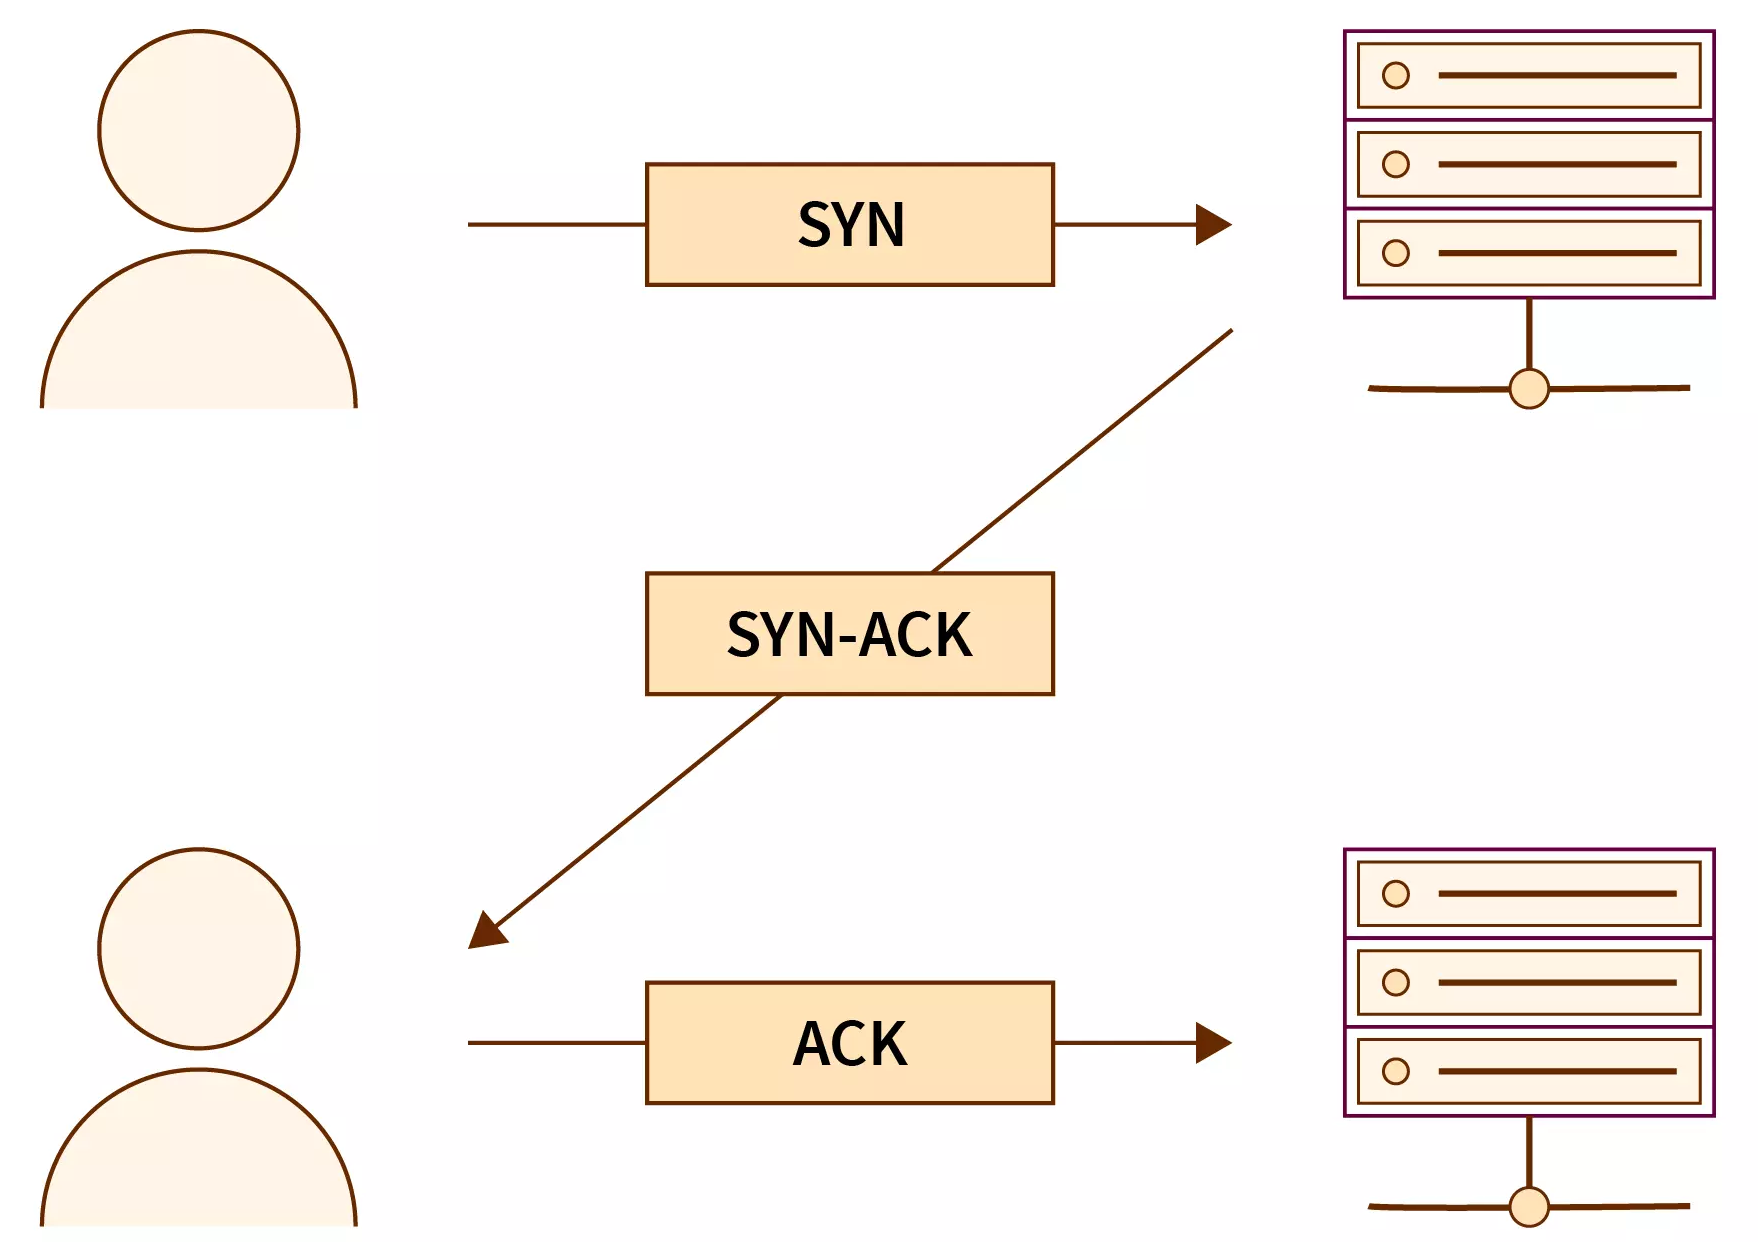
\includegraphics[width=0.8\linewidth]{figures/tcp_2wh.png}
	\caption{TCP 2-Way-Handshake}
\end{figure}

\subsection*{Segmentierung}
Es wird eine SEQUENCENUMBER mitgeschickt. Diese gibt die Reihenfolge an. Der Client bestätigt die Segmente mit ACK-Segmente. Die ACK-NUMBER gibt an, welches Segment als nächstes kommen soll.
\begin{figure}[H]
	\centering
	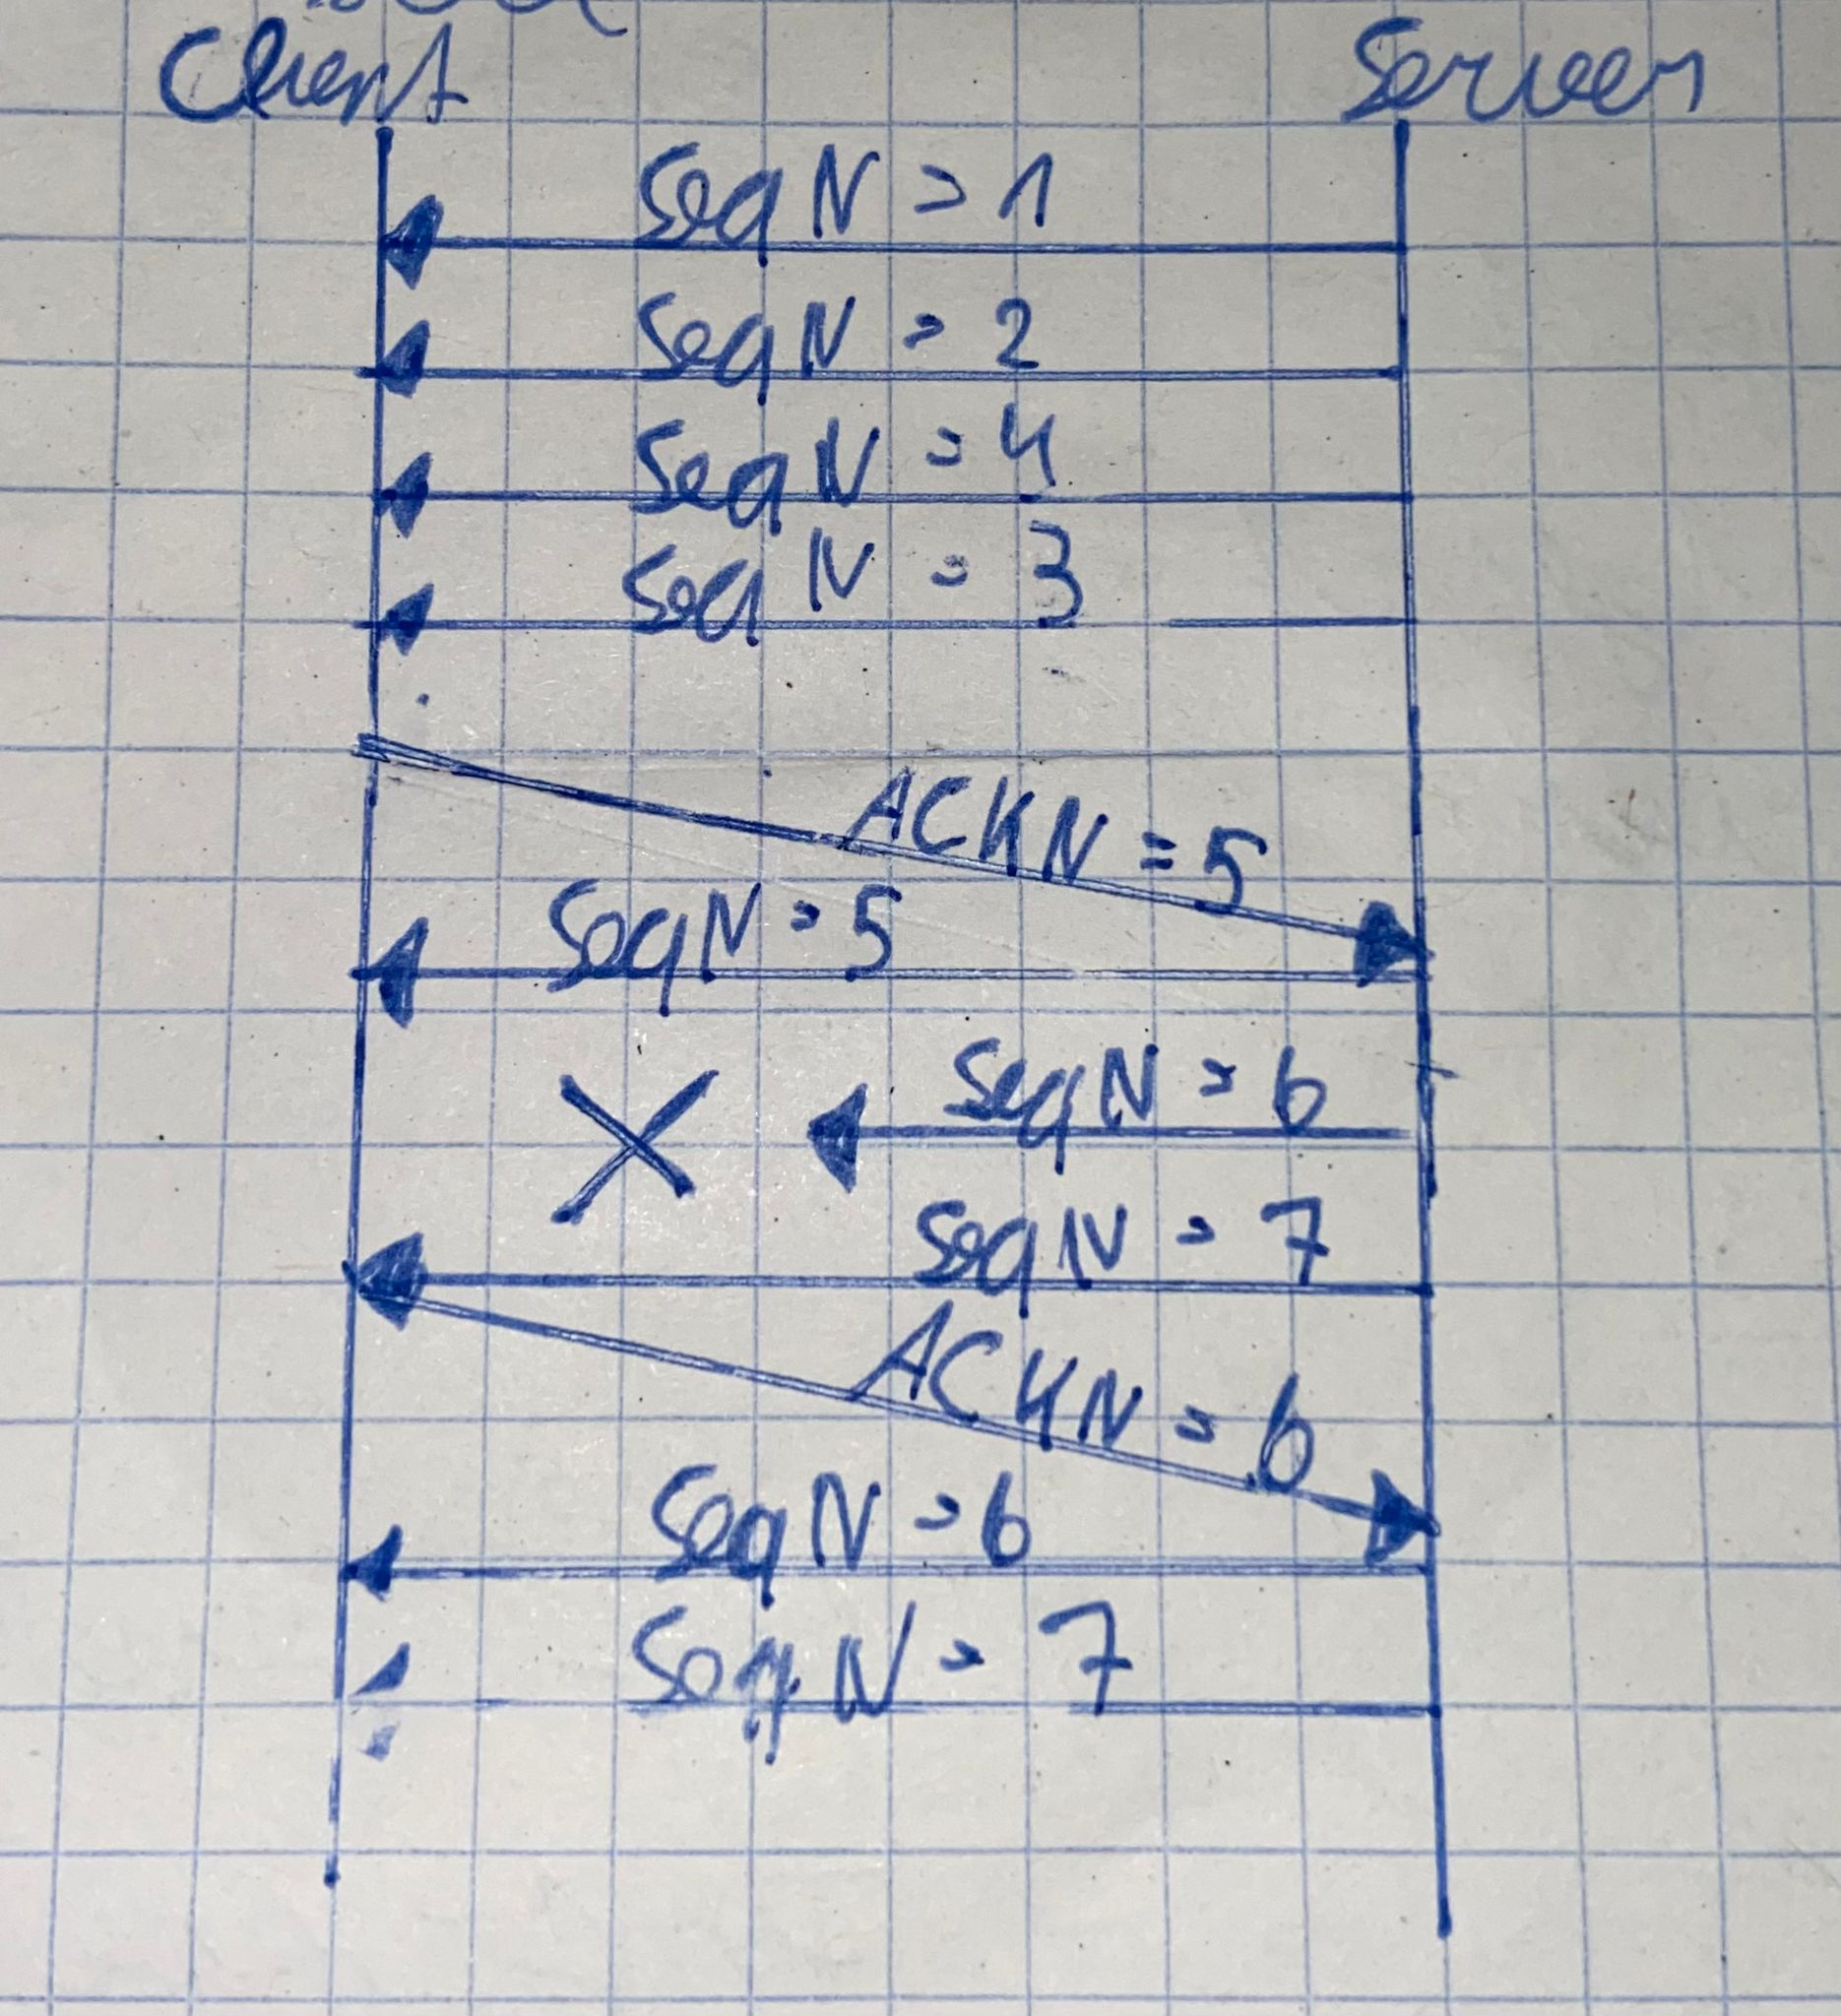
\includegraphics[width=0.8\linewidth]{figures/l4_segment.jpeg}
	\caption{Layer 4 Segmentierung}
\end{figure}

\subsection*{Flow-Control}
Die Window Size gibt an wann das nächste ACK-Segment erwartet wird.
